\documentclass[a4paper,12pt,oneside,onecolumn]{article}
\usepackage[utf8]{inputenc}
\usepackage[italian]{babel}
\usepackage{hyperref}
\usepackage[round,numbers]{natbib}
\usepackage{textcomp}
%\usepackage{listings}
%\usepackage{graphicx}
%\usepackage{amsmath}
\usepackage[T1]{fontenc}
\usepackage{lmodern}
%\usepackage[scaled=0.9]{beramono}
%\usepackage{microtype}
\usepackage{color}
\usepackage{xcolor}
%\usepackage{float}
\usepackage{lipsum}
\usepackage[noadvisor,swapnames]{frontespizio}
\usepackage{minted}
\definecolor{light-gray}{gray}{0.95}

\renewcommand*\rmdefault{iwona}

\usemintedstyle{default}

\newminted{prolog}
{ 
  frame=lines,
  framesep=2mm,
  baselinestretch=1,
  bgcolor=light-gray,
  fontsize=\small,
  linenos
}

\newminted{java}
{ 
  frame=lines,
  framesep=2mm,
  baselinestretch=1,
  bgcolor=light-gray,
  fontsize=\footnotesize,
  linenos
}

\begin{document}

    \begin{frontespizio}
        \Universita {Bari ``Aldo Moro"}
        \Logo [2cm]{./img/logo}
        \Dipartimento{Informatica}
        \Corso [Laurea]{Informatica Magistrale}
        \Titoletto {Documentazione di progetto di Intelligenza Artificiale}
        \Titolo{Sperimentazioni FOIL - ALEPH - PROGOL}
        \NCandidati{Studenti}
        \Candidato{Luciano Quercia}
        \Candidato{Simone Rutigliano}
        \Annoaccademico {2013-2014}
        \Margini{3cm}{4cm}{3cm}{3.5cm}
    \end{frontespizio}

\tableofcontents
\section{DATASETS}
\begin{table}[htbp]
	\centering
	\begin{tabular}{cccc}
		Elsevier & + 61 & Tot: 353 & \%+ 21\% \\
		 & -292 &  & \\
		 \hline
		 JMLR & +100 & Tot: 353 & \%+ 40\% \\
		 & -253 & & \\
 		 \hline
 		 MLJ & +122 & Tot: 353 & \%+ 53\% \\
 		 & -231 & & \\
 		 \hline
 		 SVLN & +70 & Tot: 353 & \%+ 25\% \\
 		 & -283 & & \\
		\end{tabular}%
	\label{tab:}
\end{table}
\subsection{ELSEVIER}
\begin{table}[htbp]
	\centering
		\begin{tabular}{cccccccccccc}
			FOLD &| &  0 &  1 &  2 &  3 &  4 &  5 &  6 &  7 &  8 &  9 \\ \hline
			Doc  &| & 35 & 35 & 35 & 35 & 35 & 35 & 35 & 36 & 36 & 36 \\
			Pos  &| & 6  & 6  &  6 &  6 &  6 &  6 &  6 &  6 &  6 &  7 \\
			Neg  &| & 29 & 29 & 29 & 29 & 29 & 29 & 29 & 30 & 30 & 29 \\
		\end{tabular}%
	\label{tab:Elsevier}
\end{table}
\subsection{JMLR}
\begin{table}[htbp]
	\centering
		\begin{tabular}{cccccccccccc}
			FOLD &| &  0 &  1 &  2 &  3 &  4 &  5 &  6 &  7 &  8 &  9 \\ \hline
			Doc  &| & 35 & 35 & 35 & 35 & 35 & 35 & 35 & 36 & 36 & 36 \\
			Pos  &| & 10  & 10  &  10 &  10 &  10 &  10 &  10 &  10 &  10 &  10 \\
			Neg  &| & 25 & 25 & 25 & 25 & 25 & 25 & 25 & 26 & 26 & 26 \\
		\end{tabular}%
	\label{tab:JMLR}
\end{table}
\subsection{MLJ}
\begin{table}[htbp]
	\centering
	%
		\begin{tabular}{cccccccccccc}
			FOLD & | &  0 &  1 &  2 &  3 &  4 &  5 &  6 &  7 &  8 &  9 \\ \hline
			Doc  & | & 35 & 35 & 35 & 35 & 35 & 35 & 35 & 36 & 36 & 36 \\
			Pos  & | & 12  & 12  &  12 &  12 &  12 &  12 &  12 &  12 &  13 &  13 \\
			Neg  & | & 23 & 23 & 23 & 23 & 23 & 23 & 23 & 24 & 24 & 24 \\
		\end{tabular}%
	
	\label{tab:MLJ}
\end{table}
\subsection{SVLN}
\begin{table}[htbp]
	\centering
		\begin{tabular}{cccccccccccc}
			FOLD &| &  0 &  1 &  2 &  3 &  4 &  5 &  6 &  7 &  8 &  9 \\\hline
			Doc  &| & 35 & 35 & 35 & 35 & 35 & 35 & 35 & 36 & 36 & 36 \\
			Pos  &| & 7  & 7  &  7 &  7 &  7 &  7 &  7 &  7 &  7 &  7 \\
			Neg  &| & 28 & 28 & 28 & 28 & 28 & 28 & 28 & 29 & 29 & 29 \\
		\end{tabular}%
	\label{tab:SVLN}
\end{table}

\section{Studio del dominio}
\nocite{AmmissionePassivo:Online}
\nocite{ChirografariCuozzo:Online}
\nocite{Curatore:Online}
\nocite{IstanzaFallimentare:Online}
\nocite{ModelliTemplate:Online}
\nocite{wiki:chirografario}
\nocite{wiki:fallimento}

%TODO Riempire di citazioni

\subsection{Il fallimento}
Il fallimento è lo strumento attraverso il quale si supera l'inattività o la volontà contraria al soddisfacimento delle obbligazioni assunte dal debitore, rispetto alle quali il suo intero patrimonio svolge una funzione di garanzia.

Si svolge nell'interesse dei creditori e nel rispetto della par condicio creditorum innanzi al Tribunale del luogo ove ha sede principale l'imprenditore.

Lo stato d'insolvenza si manifesta con inadempimenti o altri fatti esteriori, i quali dimostrino che il debitore non è più in grado di soddisfare regolarmente le proprie obbligazioni.

\subsection{Soggetti interessati}

\subsubsection{Tribunale fallimentare}
L'organo principale investito dell'intera procedura fallimentare. Nomina, revoca e sostituisce gli altri organi della procedura, quando non è prevista la competenza del giudice delegato.

\subsubsection{Imprenditore}
Sono soggetti alle disposizioni sul fallimento gli imprenditori che esercitano un'attività commerciale.

\subsubsection{Giudice delegato}
Il giudice delegato esercita funzioni di vigilanza e di controllo sulla regolarità della procedura.

\subsubsection{Curatore fallimentare}
Il curatore fallimentare è colui che ha l'amministrazione del patrimonio fallimentare e compie tutte le operazioni della procedura fallimentare sotto la vigilanza del giudice delegato e del comitato dei creditori, nell'ambito delle funzioni ad esso attribuite.


\subsubsection{Comitato dei creditori}
Il comitato dei creditori vigila sull'operato del curatore e ne propone la revoca, autorizza gli atti, esprime pareri.
I membri possono svolgere ispezioni sulle scritture contabili e sui documenti della procedura. È nominato dal giudice delegato, sentiti il curatore e i creditori stessi.


\subsection{Istanza di fallimento}
L'istanza di fallimento è l'atto attraverso il quale viene richiesto alla Pubblica Autorità di aprire una procedura fallimentare nei confronti di un determinato imprenditore.

Può essere presentata da:
\begin{itemize}
\item il debitore stesso che chiede il proprio fallimento; 
\item i creditori di un soggetto insolvente; 
\item il pubblico ministero. 
\end{itemize}

\subsection{Iscrizione al passivo}
Qualunque soggetto sia creditore di un imprenditore fallito ha diritto ad insinuarsi al passivo del fallimento, così da poter concorrere, insieme agli altri creditori insinuati, per ottenere il soddisfacimento del proprio credito nell'ambito del fallimento.

\subsubsection{Tipologia di iscrizione}
\label{Tipologia di iscrizione}
Se il credito è assistito da un privilegio (come ad esempio il pegno o l’ipoteca) ha diritto ad essere soddisfatto con precedenza sugli altri creditori non privilegiati; se invece non è assistito da privilegio si dice creditore "chirografario", il cui credito può essere soddisfatto solo e nella misura in cui vi sia un residuo dell'attivo fallimentare dopo il soddisfacimento dei creditori privilegiati. 
Con la domanda di ammissione al passivo, quindi, il creditore presenta agli organi del fallimento la propria domanda di insinuazione al passivo, ovvero di essere incluso nel novero dei creditori che concorreranno alla distribuzione dell'attivo del fallimento.

\subsubsection{Modelli di iscrizione al passivo}

Di seguito verranno mostrati tre \emph{facsimile} di moduli di iscrizione al passivo, reperiti su web, su siti di modulistica di tribunali.

\begin{figure}[H]
\centering
\fbox{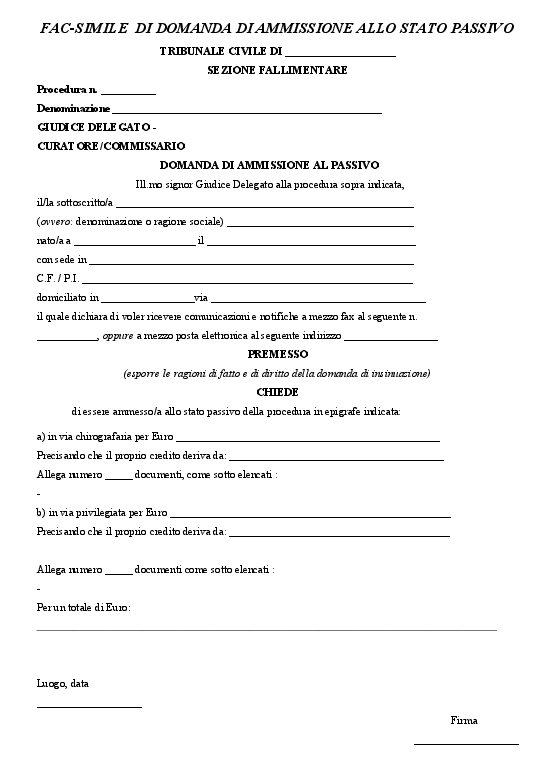
\includegraphics[width=.9\textwidth]{img/2.png}}
\caption{Fac-simile di domanda di ammissione allo stato passivo.}
\label{fig:modello1}
\end{figure}

\begin{figure}[H]
\centering
\fbox{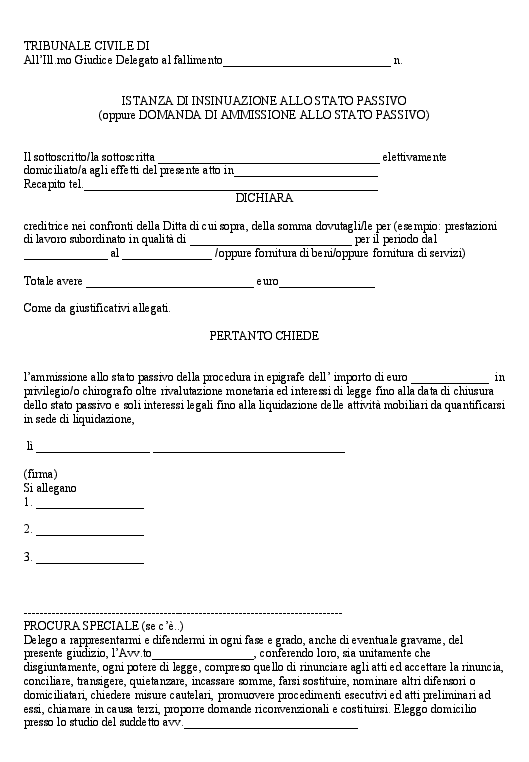
\includegraphics[width=.9\textwidth]{img/3.png}}
\caption{Istanza di insinuazione allo stato passivo.}
\label{fig:modello2}
\end{figure}

\begin{figure}[H]
\centering
\fbox{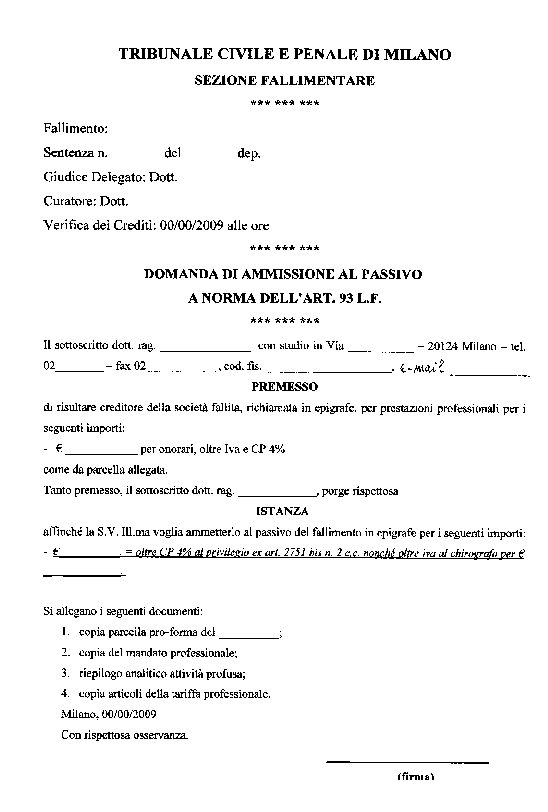
\includegraphics[width=.9\textwidth]{img/1.png}}
\caption{Modello di iscrizione al passivo pubblicato online dal Tribunale di Milano.}
\label{fig:modello3}
\end{figure}


\subsection{Individuazione dei bisogni dell’utente}
A causa della scarsa informatizzazione dei Tribunali (come purtroppo della maggior parte delle strutture pubbliche in Italia), i moduli da presentare ad ogni livello della procedura sono in forma cartacea, basati su modelli spesso diversi tra loro.

Ad esempio, la fig.~\ref{fig:modello3} mostra il modello pubblicato e liberamente scaricabile dal sito del Tribunale Civile e Penale di Milano \cite{milano:modulistica}.

Come è facile intuire, la presenza di diversi modelli, unita al numero elevato di documenti da esaminare, rende oneroso il compito del curatore fallimentare.

Per semplificare il lavoro sarebbe utile uno strumento in grado di estrarre in maniera automatica le informazioni necessarie al curatore, indipendentemente dal template utilizzato.

\section{Progettazione}

\label{sec:Progettazione}

\subsection{Obiettivo}
Come primo obiettivo, il sistema deve essere in grado di estrarre, da documenti testuali, alcune informazioni principali, quali:
\begin{itemize}
\item numero della pratica;
\item soggetto della richiesta di iscrizione;
\item quantità di denaro richiesta e tipologia.
\end{itemize}

Come feature aggiuntive, il sistema si può occupare dell'estrazione, su richiesta, di altre informazioni utili come:
\begin{itemize}
\item indirizzi email;
\item numeri di telefono;
\item nomi di comuni;
\item altre persone nominate nel testo;
\item etc.
\end{itemize}

\subsection{Input e Assunzioni}
Non avendo a disposizione dei documenti di input reali sui quali il sistema deve essere in grado di lavorare e, quindi, non conoscendone il formato o la composizione, abbiamo dovuto fare delle assunzioni e realizzare degli esempi di input \emph{ad-hoc}.
Per essere pronti a successivi adattamenti, abbiamo fatto le scelte meno vantaggiose, ipotizzando di non avere a disposizione alcuna strutturazione nel documento o metadati su di esso.

I nostri esempi di input sono delle semplicissime stringhe prive di tabulazioni, ordinamento nello spazio, tag di qualsiasi tipo.

Nel caso in cui in futuro dovessimo essere in possesso di alcune di queste informazioni, potremmo utilizzarle per migliorare le nostre regole.


\subsection{Strategia risolutiva}
Il problema che affronteremo rientra nell'ambito dell'\emph{Information Extraction}, un task di Intelligenza Artificiale che mira all'estrazione automatica di informazioni strutturate da documenti non-strutturati o semi-strutturati.

Nella maggior parte dei casi, questa attività riguarda l'elaborazione di testi scritti in linguaggio naturale (NLP).

Abbiamo deciso di servirci di alcune delle tecniche di analisi lessicale e sintattica già note e utilizzate in questo campo.

\subsubsection{Lexical Analysis}
Il testo in input (come già detto testo semplice in una stringa) subisce una pre-elaborazione lessicale, con l'obiettivo di ottenere una lista di token da passare al tagger (\ref{tagger}).

Questa pre-elaborazione principalmente si occupa di:
\begin{itemize}
\item eliminare i caratteri \emph{inutili} per i nostri scopi quali, ad esempio \verb+!+, \verb+?+;
\item normalizzare tutte le lettere in minuscolo.
\item eliminare le \emph{stopword}, ossia delle parole come congiunzioni, interiezioni o avverbi inutili al nostro scopo.
\end{itemize}


\subsubsection{Creazione dei token}
Dopo l'elaborazione descritta nella sezione precedente, il sistema si occupa di creare un identificatore per ogni token, nella forma \verb:`tok'+Num: con \verb+Num+ intero positivo crescente.

Per ognuno dei token trovati, verranno asseriti alcuni fatti che rappresentano la base di conoscenza sulla quale le regole cercheranno i vari tag ai quali siamo interessati.

Di seguito un esempio esplicativo dei fatti asseriti.

\begin{prologcode}
token('tok1', 'curatore').
token('tok2', 'fallimentare').
token('tok3', 'tribunale').
token('tok4', 'milano').
next('tok1', 'tok2').
next('tok2', 'tok3').
next('tok3', 'tok4').
\end{prologcode}

\subsubsection{Gestione di più documenti}
Il sistema è in grado di lavorare su diversi documenti di input senza problemi.

Per farlo abbiamo introdotto un nuovo predicato, \verb+appartiene/2+ e due nuovi token per ogni documento: \verb+BOF+ e \verb+EOF+.
Ad ogni documento passato in input, viene assegnato un identificatore, nella forma \verb:`doc'+Num:. Inoltre vengono generati due nuovi token fittizi, chiamati BOF (Begin Of File) e EOF (End Of File), rispettivamente token di inizio e file documento.

Per ognuno dei token ritrovati nella stringa del documento, oltre ai 2 fittizi, viene inoltre asserita l'appartenenza al documento.

Nel pezzo di codice seguente sono riportati degli esempi.

\begin{prologcode}
documento('doc0', "Questo è un esempio").
token('tok1', 'doc0_BOF').
token('tok1', 'doc0_EOF').
appartiene('tok1', 'doc0').
appartiene('tok2', 'doc0').
appartiene('tok3', 'doc0').
appartiene('tok4', 'doc0').
appartiene('tok5', 'doc0').
\end{prologcode}





Il tagger è la componente che lavora sulle liste di token precedentemente create, alla ricerca di pattern noti per poter assegnare una semantica ai token. In questo modo si andranno a individuare gli oggetti del dominio contenuti all'interno del documento da analizzare.

\subsection{Oggetti del dominio}
Per poter estrarre le informazioni a più alto livello quali, ad esempio, \emph{soggetto} e \emph{quantità di denaro richiesta}, dobbiamo utilizzare numerosi oggetti, specifici del dominio giuridico e non.

\subsubsection{Persone}
Per l'individuazione delle persone fisiche presenti nel testo (oltre al soggetto della richiesta, anche il giudice, l'avvocato o altre persone nominate nel testo) è utile riuscire a distinguere un \fbox{nome} e un \fbox{cognome}, eventuali \fbox{titoli} che riescono a contraddistinguere il ruolo della persona fisica all'interno del testo.

\subsubsection{Richiesta di denaro}
Per quanto riguarda invece la ricerca del quantitativo di denaro che il soggetto della richiesta dovrà ottenere, diventa necessario individuare in primis il \fbox{valore} e successivamente anche la \fbox{tipologia} della richiesta di rimborso, quindi se chirografata o privilegiata cosi come detto in precedenza nel paragrafo \ref{Tipologia di iscrizione}.

\subsubsection{Oggetti aggiuntivi}
Sono state estratte anche altre informazioni aggiuntive che potrebbero rivelarsi utili all'utilizzatore del sistema, quali ad esempio eventuali email, date, nomi di comuni, codici fiscali e anche numeri di telefono presenti all'interno del documento.

\subsection{Individuazione delle relazioni}
%TODO Fa Luciano

% !TeX encoding = UTF-8
% !TeX spellcheck = it_IT
% !TeX root = main.tex

\section{Implementazione}

\subsection{Architettura del sistema}
Per preservare l'indipendenza delle componenti del sistema, abbiamo realizzato dei moduli Prolog che espongano pubblicamente solo i predicati necessari.

Il file \verb+main.pl+ costituisce l'entry-point del programma, l'unico file necessario da importare nell'interprete per l'esecuzione.


\subsection{Lexer}
Il compito del \emph{lexer} sarà quello di normalizzare la stringa contenente il documento da analizzare in una lista di token su cui poi il tagger dovrà fare le sue analisi. Per fare ciò, bisognerà nell'ordine:
\begin{itemize}
    \item ripulire la stringa di stopchars;
    \item separare i caratteri speciali (punto, virgola, euro e chiocciola) da eventuali caratteri a cui sono associati;
    \item eliminare eventuali spazi bianchi superflui causati da eliminazioni di caratteri fatte in precedenza;
    \item rendere case insensitive la stringa ripulita.
\end{itemize}

Per quanto riguarda la pulizia degli stopchar ininfluenti ai fini del tag, si è deciso di eliminare i caratteri quali il punto interrogativo, il punto esclamativo, virgolette, apici, punti e virgola, due punti e parentesi tonde e graffe.

Alcuni caratteri speciali sono stati preservati e separati dai token a cui sono uniti in modo da diventare essi stessi dei nuovi token. Questo perché tali caratteri hanno una semantica in alcune regole di livello più alto.
Ad esempio il carattere speciale euro (€) risulta essere molto utile per l'identificazione di richieste di denaro all'interno del documento.

Di seguito, a titolo esemplificativo, il codice del predicato lexer:

\begin{prologcode}
lexer(String, ListToken) :-
   strip_useless_chars(String, Temp1),
   separate_useful_chars(Temp1, Temp2),
   strip_spaces(Temp2, Temp3),
   atom_codes(Temp4, Temp3),
   atomic_list_concat(Temp5, ' ', Temp4),
   maplist(downcase_atom, Temp5, Temp6),
   strip_sep(Temp6, ListToken).
\end{prologcode}

\subsection{Creazione dei token}
\label{sec:creazionetoken}
Dopo l'elaborazione descritta nella sezione precedente, il sistema si occupa di creare un identificatore per ogni token, nella forma \verb:tok<Num>: con \verb+<Num>+ intero positivo crescente.

Per ognuno dei token trovati, verranno asseriti alcuni fatti che rappresentano la base di conoscenza sulla quale le regole cercheranno i vari tag ai quali siamo interessati.

Di seguito un esempio esplicativo dei fatti asseriti.

\begin{prologcode}
token('tok1', 'curatore').
token('tok2', 'fallimentare').
token('tok3', 'tribunale').
token('tok4', 'milano').
next('tok1', 'tok2').
next('tok2', 'tok3').
next('tok3', 'tok4').
\end{prologcode}


\subsection{Gestione di più documenti}
Il sistema è in grado di lavorare su diversi documenti di input senza conflitti o interazioni.

Per farlo abbiamo introdotto un nuovo predicato, \verb+appartiene/2+ e due nuovi token per ogni documento: \verb+BOF+ e \verb+EOF+.
Ad ogni documento passato in input, viene assegnato un identificatore, nella forma \verb:doc<Num>:. Inoltre vengono generati due nuovi token fittizi, chiamati \verb+BOF+ (Begin Of File) e \verb+EOF+ (End Of File), rispettivamente token di inizio e file documento.

Per ognuno dei token ritrovati nella stringa del documento, oltre ai 2 fittizi, viene inoltre asserita l'appartenenza al documento.

Nel pezzo di codice seguente sono riportati degli esempi.

\begin{prologcode}
documento('doc0', "Questo e' un esempio").
token('tok0', 'doc0_BOF').
token('tok5', 'doc0_EOF').

appartiene('tok0', 'doc0').
appartiene('tok1', 'doc0').
appartiene('tok2', 'doc0').
appartiene('tok3', 'doc0').
appartiene('tok4', 'doc0').
appartiene('tok5', 'doc0').

next('tok0', 'tok1').
next('tok4', 'tok5').
\end{prologcode}

\subsection{Creazione dei tag}
Dopo che tutte le informazioni sui documenti e sui token in input sono state elaborate ed asserite, intervengono delle regole che asseriscono i \verb|tag|, ossia dei token specializzati dotati di semantica.

La ricerca dei \verb|tag| avviene a livelli successivi:
per poter identificare un tag più complesso, il sistema ha bisogno di individuare \verb|tag| più semplici.

La gerarchia delle dipendenze è mostrata in figura \ref{fig:dipendenze}


\begin{figure}[H]
\centering
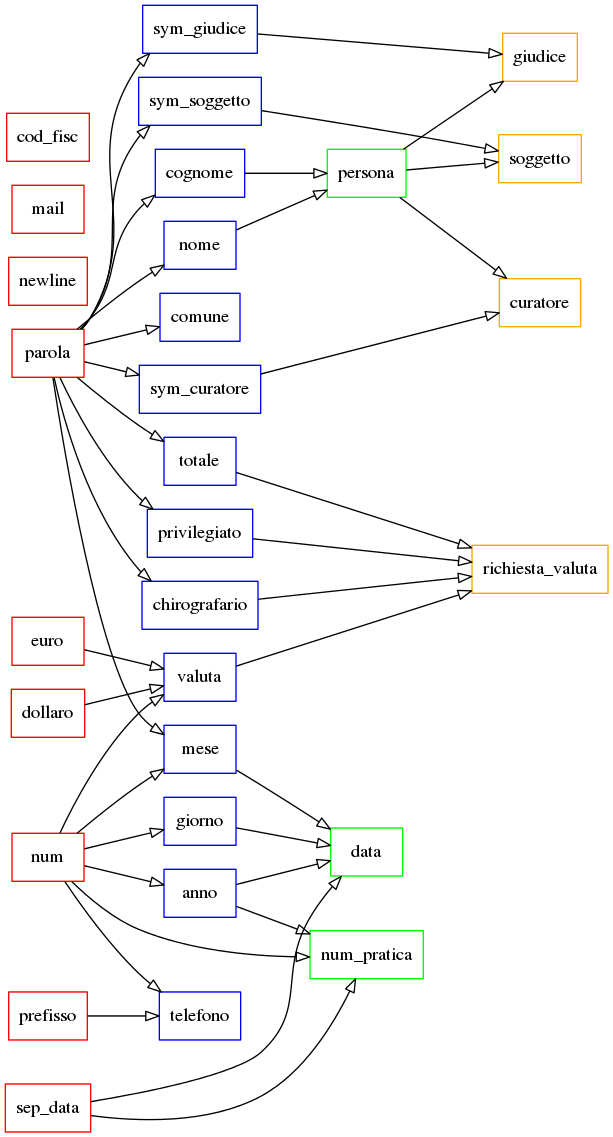
\includegraphics[width=.8\textwidth]{img/dipendenze.png}
\label{fig:dipendenze}
\caption{Schema delle dipendenze esistenti tra tag}
\end{figure}

In figura \ref{fig:dipendenze}, in \verb|tag| di colore rosso rappresentano il livello più basso, cioè i \verb|tag| riconoscibili a partire dai \verb|token| tramite analisi sintattica e espressioni regolari.

I \verb|tag| di colore blu utilizzano quelli del livello precedente per identificare nuove entità. Similmente succede per gli altri due livelli.

\subsubsection{Come funziona il tagger}

Similmente a quanto descritto a pagina \pageref{sec:creazionetoken} per i token, per ogni nuovo \verb|tag| viene creato un identificatore, nella forma \verb:tag<Num>: con \verb+<Num>+ intero positivo crescente.

Nell'ordine:
\begin{enumerate}
\item Viene asserito il nuovo tag tramite il predicato \verb|tag/2|;
\item Viene confermata l'appartenenza allo stesso documento dei \verb|token|/\verb|tag| dai quali deriva tramite il predicato \verb|appartiene/2|;
\item si asserisce la vicinanza (predicato \verb|next/2|) tra tutti i \verb|token|/\verb|tag| che precedono quelli dai quali deriva il \verb|tag| corrente e il \verb|tag| corrente;
\item si asserisce la vicinanza (predicato \verb|next/2|) tra il \verb|tag| corrente e tutti i \verb|token|/\verb|tag| che succedono a quelli dai quali deriva il \verb|tag| corrente;
\end{enumerate} 

Il codice seguente esemplifica alcune delle asserzioni del tagger in un documento composto da due parole: ``curatore fallimentare''.

\begin{prologcode}
token(tok0, BOF).
token(tok1, curatore).
token(tok2, fallimentare).
token(tok3, EOF).

tag(tag0, parola(curatore)).
next(tok0, tag0).
next(tag0, tok2).

tag(tag1, parola(fallimentare)).
next(tok1, tag1).
next(tag0, tag1).
next(tag1, tok3).
\end{prologcode}

La figura seguente invece, mostra invece tutti gli archi \verb|next| che vengono creati nel tagging di un documento composto dalle parole: ``Luigi Nesta''.

\begin{figure}[H]
\centering
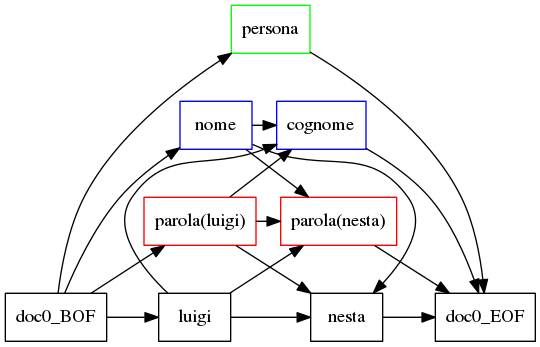
\includegraphics[width=\textwidth]{img/nuovitag.png}
\label{fig:nuovitag}
\caption{Schema dei \emph{next/2} in un documento composto dalle parole ``Luigi Nesta''.}
\end{figure}

% !TeX encoding = UTF-8
% !TeX spellcheck = it_IT
% !TeX root = main.tex

\section{Componenti aggiuntive}
Il sistema oltre a fornire i servizi di base necessari a soddisfare l'obiettivo prefissato definito nella sezione \ref{object}, presenta alcune funzionalità aggiuntive atte a migliorare l'esperienza con il sistema. Tra queste funzionalità aggiuntive, le principali sono:
\begin{itemize}
	\item Modulo di spiegazione
	\item Interfaccia grafica Java
	\item Rappresentazione visuale delle spiegazioni tramite graphviz
\end{itemize}
Di seguito verrà fatta una breve descrizione per ogni funzionalità.

\subsection{Modulo di spiegazione}
\label{spiega}
Il sistema, una volta terminata l'elaborazione e mostrato a video i risultati del tag, da la possibilità all'utilizzatore di capire come è stato possibile etichettare quel gruppo di parole in un determinato tag. Per fare ciò, durante l'elaborazione, il sistema man mano che cerca di etichettare un particolare tag (ad esempio \emph{Persona}), asserisce oltre ai vari IDDoc, ListaPrecedenti, ListaSuccessivi, etc. , anche la spiegazione di come si è raggiunto quel particolare tag.

Ad esempio, in caso di tag di persone, all'interno del predicato \emph{tag\_persone}, sarà presente anche:

\begin{prologcode}
 tag_persona(C, N) :-
   ...
   atomic_list_concat(['[PERSONA] Presenza nel documento di:',C,N],
                      ' ',Spiegazione),
   ...
   assertTag(persona(C, N),IDDoc, ListaPrecedenti, ListaSuccessivi,
            Spiegazione, Dipendenze).
\end{prologcode}

Successivamente, qualora l'utente dovesse richiedere la spiegazione di un particolare tag, il sistema, indipendentemente dall'interfaccia utilizzata (per i diversi tipi di approcci interattivi vedere cap. \ref{Interaction}), non farà altro che richiamare il predicato \emph{spiega\_tutto} il cui compito sarà quello di recuperare tutte le spiegazioni dei vari sottotag che compongono il tag di cui si vuole ottenere la spiegazione.
Ad esempio, se nel documento è presente una frase del tipo : \emph{... Richiesta in via chirografaria di 2000\officialeuro ...} , in questo il sistema creerà un tag \emph{richiesta\_valuta(2000, euro, chirografario)}.

Qualora volessimo sapere il come è stato creato questo tag, il sistema risponderà nel seguente modo:

\begin{verbatim}
[RICHIESTA VALUTA] Presenza nella stessa frase della valuta 2000
                   euro e del termine chirografaria
[TIPO_RICHIESTA] Presenza nel documento del termine chirografaria
[VALUTA] Presenza nel documento del numero 2000 preceduto dal 
         simbolo €
\end{verbatim}
\subsection{Interfaccia grafica Java}
Tra le feature aggiuntive offerte dal sistema, vi è la presenza di un'interfaccia grafica creata in Java utile al fine di poter migliorare l'usabilità del sistema permettendone l'utilizzo anche a chi non è molto pratico di interfacce a linee di comando. Nel capitolo \ref{Interaction} verrà descritto in dettaglio come si presenta l'interfaccia grafica e un suo esempio di interazione. 
Per permettere la realizzazione delle interfacce grafiche in Java è stato, inoltre, necessario far comunicare Prolog con Java in modo tale da poter permettere uno scambio di informazioni tra i due sistemi; per fare ciò sono state utilizzate due librerie Java nate per questo scopo quali JPL e InterProlog di cui si parlerà approfonditamente rispettivamente nelle sezioni \ref{JPL} e \ref{InterProlog}.
\subsection{Rappresentazione visuale tramite graphviz}
\nocite{gansner2006drawing}
\nocite{wiki:Graphviz}
Un'ulteriore feature offerta dal sistema è quella inerente al modo con cui visualizzare le spiegazioni dei tag che il sistema ha creato; in particolare, oltre alla spiegazione testuale cosi come mostrata nella sezione \ref{spiega}, il sistema offre un'immagine che mostra in maniera grafica come è stato ottenuto il tag.
Prendendo come esempio il tag \emph{richiesta\_valuta} descritto nella sezione \ref{spiega}, la visualizzazione grafica di quel tag sarà:

\begin{figure}[H]
	\centering
	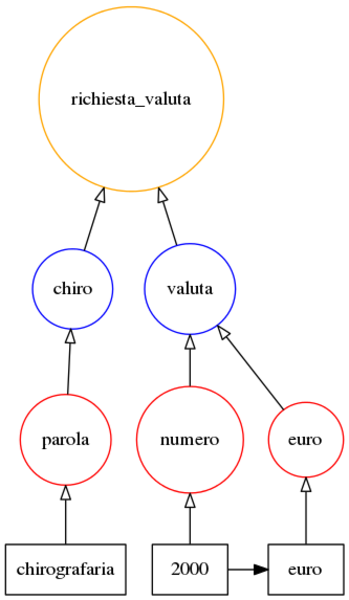
\includegraphics[width=0.5\textwidth]{img/tagRichiesta.png}
	\caption{Esempio spiegazione richiesta\_valuta}
\end{figure}

Per poter ottenere un grafico di questo tipo, è stato necessario utilizzare un programma open source chiamato \emph{Graphviz} (abbreviazione di Graph Visualization Software), il quale è in grado di disegnare grafi descritti nel linguaggio \emph{DOT}.

Il linguaggio \emph{DOT} è un linguaggio di descrizione di grafi in plain text, inoltre, l'utilizzo di questo linguaggio rende più semplice descrivere i grafi dato che sono facilmente usabili sia dall'essere umano che dalla macchina. I grafi descrivibili da questo linguaggio possono essere sia grafi orientati che non; nel nostro caso è stato necessario garantire la direzionalità dell'arco.
\clearpage
Un esempio di codice dot per descrivere un grafo orientato (\emph{V},\emph{E}), dove 
$$V = \left\{ a,b,c \right\} $$
$$E = \left\{ \left( a,b \right) , \left( b,c \right) , \left( b,d \right) \right\} $$
è il seguente:

\begin{verbatim}
	digraph graphExample {
	    a -> b -> c;
	    b -> d;
	}
\end{verbatim}
Dove la parola chiave \emph{digraph} indica che il grafo che si andrà a creare sarà orientato (Directed), mentre \emph{graphExample} sarà il nome del grafo da creare.
Una volta creato il file .dot sarà necessario processarlo dall'omonimo programma al fine di poter ottenere l'immagine in formato PNG da poter visualizzare.
Il comando da terminale da dover usare per la creazione dell'immagine in formato PNG sarà il seguente:
\begin{verbatim}
  dot -Tpng ./graphExample.dot > ./graphExample.png
\end{verbatim}

L'output dell'immagine creata dal dot sarà:
\begin{figure}[H]
	\centering
	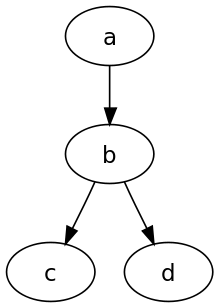
\includegraphics[width=0.4\textwidth]{img/220px-DotLanguageDirected.png}
	\caption{Esempio di grafo dot}
\end{figure}
\section{Descrizione del sistema}

Il sistema presenta un'interfaccia grafica in grado di permettere l'interazione con il core del sistema scritto in Prolog, dando cosi la possibilità a qualunque tipo di stakeholders del sistema di utilizzarlo senza la necessità di dover interagire con il terminale, rendendo cosi le informazioni più leggibili e usabili; Oltre a questo, la creazione dell'interfaccia permette anche di evitare possibili errori dattilografici che si potrebbero avere in caso di interazione con il terminale.

Gli elementi principali dell'interfaccia, con i relativi pulsanti, la cui funzione e uso verranno descritti in dettaglio nel prossimo paragrafo, sono i seguenti (nella figura %TODO
i numeri delle aree corrispondono alle rispettive funzioni assegnate enumerate
nell'elenco seguente):
\begin{itemize}
  \item Sezione di inserimento del documento da cui si devono estrarre le informazioni;
  \item Sezione di scelta delle informazioni da estrarre;
  \item Sezione di visualizzazione dei risultati ottenuti.
\end{itemize}
\subsection{Sezioni ed operazioni disponibili}
    \subsubsection{Inserimento}
    \label{Inserimento}
    In questa sezione viene data la possibilità di inserire il documento testuale da cui si vogliono estrarre le informazioni; con questa operazione non si fa altro che asserire un documento da dover poi essere processato dal core prolog del sistema.
    \subsubsection{Scelta dei tag}
    \label{ChoiceTag}
    In questa sezione si da la possibilità all'utente di filtrare i tag da voler estrarre dal documento attraverso la selezione/deselezione della checkbox corrispondente al tag; con questa operazione si vanno a selezionare quali saranno i tag che il core prolog deve etichettare nel documento.
    \subsubsection{Visualizzazione}
    \label{Visualization}
    In questa schermata invece verranno mostrate le informazioni che l'utente ha deciso di estrarre dal documento; inoltre le diverse tipologie di tag saranno evidenziate diversamente l'uno dall'altro attraverso l'ausilio di una colorazione dei tag. 

    \subsubsection{Reset delle condizioni iniziali}
    Tramite il pulsante \emph{Reset} si ripristinano le condizioni iniziali del sistema.In particolare, viene ripristinato lo stato iniziale:
    \begin{itemize}
      \item \emph{Interfaccia} : cancellando le textbox contenenti il documento inserito \ref{Inserimento} e i tag etichettati dal testo \ref{Visualization}, sia le scelte dei tag da effettuare \ref{ChoiceTag}.
      \item \emph{Core Prolog} : ritrattando il documento appena inserito nella sezione \ref{Inserimento}.
    \end{itemize}
    
\subsection{Interazione con l'utente}
L’interazione avviene principalmente tramite l'interfaccia grafica descritta nella sezione precedente ma viene data anche la possibilità di interagire con il sistema anche senza l'ausilio di tale interfaccia, utilizzando direttamente l'interprete Prolog da terminale, previa consultazione del modulo principale del sistema denominato \emph{main.pl}; le funzionalità del sistema sono indipendenti dal metodo con cui si vuole interagire con il  sistema. Qualora si volesse tener traccia anche di come avviene la comunicazione tra java e prolog, è possibile visionare tale interazione all'interno della finestra di terminale da cui si è lanciato il sistema.

\subsection{Comunicazione Java Prolog}
\subsubsection{JPL Library}
\nocite{swi:jpl}
La libreria utilizzata per permettere la bidirezionalità della comunicazione tra Java e Prolog, è stata la \emph{JPL 3.1.4 alpha}\footnote{Scaricabile da \url{http://mvnrepository.com/artifact/jpl/jpl/3.1.4-alpha}} (\textbf{J}ava-calls-\textbf{P}rolog \textbf{L}ibrary)

Le API messe a disposizione dalla libreria JPL permettono la creazione di oggetti Java che andranno a inglobare gli elementi che saranno poi utilizzati lato Prolog. La struttura gerarchica delle classi presenti nella libreria è la seguente:
\begin{Verbatim}
Term
|
+--- Variable
|
+--- Compound
|      |
|      +--- Atom
|
+--- Integer
|
+--- Float

Query

JPLException
|
+-- PrologException
\end{Verbatim}

Le classi Term-based sono in grado di adattare al meglio la concreta sintassi strutturata dei termini di Prolog, in quanto non esiste una corrispondenza diretta con un particolare termine di Prolog; piuttosto, esistono diversi significati assunti dalla classe Term, si va dalla necessità di creare delle strutture da essere utilizzate all'interno di query Prolog, fino ad arrivare al tipo di rappresentazione, con relativa esplorazione, dei risultati ottenuti dalla query.
Per astrarre quindi il concetto di termine, la classe \emph{Term} è una classe astratta istanziata da una delle sue cinque possibili sottoclassi:
\paragraph{Compounds}
Un Compound è un Termine che contiene un nome e una sequenza di argomenti di tipo Term.

\begin{javacode}
Compound teacher_of = new Compound("teacher_of",
                  new Term[] {
                        new Atom("aristotle"),
                        new Atom("alexander")
                        }
                );
\end{javacode}

In questo esempio, la variabile java \emph{teacher\_of} si riferisce a una istanza di tipo \emph{Compound} che rappresenta il termine prolog.

\begin{prologcode}
  teacher_of(aristotle,alexander).
\end{prologcode}

\paragraph{Atom}
Un Atom è una specializzazione di \emph{Compound} avente zero parametri, il che vorrà dire che Atom sarà un Term contenente solo un nome.

\begin{javacode}
Atom aristotle = new Atom("aristotle");
Atom alexander = new Atom("alexander");
\end{javacode}

\paragraph{Variable}
Le Variabili sono dei Term aventi un nome identificativo il quale deve soddisfare la sintassi Prolog.

\begin{javacode}
Variable X = new Variable("X");  //  variabile X
Variable X = new Variable("_");  //  variabile "anonima"
Variable X = new Variable("_Y"); // variabile Y di cui non si vuole 
                 // conoscere il contenuto
\end{javacode}

\paragraph{Integer}
Un Integer è una specializzazione di \emph{Term} che mantiene la valorizzazione di tipo long di Java. Questa classe corrisponde al tipo integer di Prolog.

\begin{javacode}
jpl.Integer i = new jpl.Integer(5);
\end{javacode}

\paragraph{Floats}
Un Float è una specializzazione di \emph{Term} che mantiene la valorizzazione di tipo double di Java. Questa classe corrisponde al tipo float di Prolog sulla quale possono essere eseguite le operazioni aritmetiche.

\begin{javacode}
  jpl.Float f = new jpl.Float(3.14159265);
\end{javacode}

\paragraph{Queries}
Ogni istanza di Query contiene un \emph{Term}, il quale rappresenta il goal da dimostrare.

\begin{javacode}
  Term goal = new Compound("teacher_of",
    new Term[] {
        new Atom("aristotle"),
        new Atom("alexander")
        }
  );
  Query q = new Query( goal );
\end{javacode}

La query q in questo esempio rappresenta la query Prolog:

\begin{prologcode}
  ?- teacher_of(aristotle,alexander).
\end{prologcode}

\subsubsection{Funzionamento}
Per garantire l'interazione tra Java e Prolog, le principali istruzioni utilizzate per permettere questa comunicazione, sono state le seguenti:

\begin{javacode}
  JPL.setNativeLibraryDir("/usr/local/lib/Yap");
  prolog.consult(new Atom("prolog/main.pl"));
  prolog.retractAll("domanda", 1);
  Term toAssert = new Compound("domanda", 
                  new Term[]{
                     Util.textToTerm("\"" + textPane.getText() + "\"")}
                  );
  prolog.asserta(toAssert);
  java.util.Hashtable<String, Term>[] hashtables = null;
  hashtables = prolog.allSolutions(new Compound("nextTag", 
                                  new Term[]{
                                      new Variable("Tag")})
                                      );  
\end{javacode}
\paragraph{inizialize}
I primi comandi hanno il compito di inizializzare il motore Prolog definendo 
\begin{itemize}
    \item Quali librerie utilizzare per la dimostrazione del goal (in questo caso si è deciso di utilizzare le librerie di \emph{Yap});
    \item Definire la base di conoscenza tramite i consult, i retract e gli assert, sia dei fatti che delle regole da utilizzare.
\end{itemize}
Il codice java atto a realizzare sia la consult che la retract è il seguente:

\begin{javacode}
  public boolean consult(Atom atom) {
    Term t = new Compound("consult", new Term[]{atom});
    Query query = new Query(t);
    System.out.print("[Prolog] consult: " + t + " ");
    System.out.println(query.hasSolution() ? "succeeded" : "failed");
    return query.hasSolution();
  }
\end{javacode}

\begin{javacode} 
 public void retractAll(String predicate, int arity) {  
   Term[] args = new Term[arity];
   for (int i = 0; i < args.length; i++)
       args[i] = new Variable("_");
   Term[] termToRetract = new Term[]{ new Compound(predicate, args) };    
   Term t = new Compound("retractall", termToRetract);
   Query query = new Query(t);
   System.err.print("[Prolog] retract( " + predicate + " ) ");
   System.err.println(query.hasSolution() ? "succeeded" : "failed");
 }
\end{javacode}

\paragraph{Queries}
Una volta ultimata l'inizializzazione, il passo successivo sarà quello di estrarre i risultati del tag che il sistema ha prodotto; per fare ciò, verranno create delle query parametrizzate adeguatamente da Termini e i risultati verranno inseriti all'interno di un array di tipo Hashtable.

\begin{javacode}
 public java.util.Hashtable[] allSolutions(Term t) {
   Query query = new Query(t);
   System.err.print("[Prolog] query: " + t + " ");
   System.err.println(query.hasSolution() ? "succeeded" : "failed");
   return query.allSolutions();
 }
\end{javacode}

\subsection{Esempio di interazione}

\subsection{Presentazione dei risultati}

\subsection{Utilizzo della funzione spiega ragionamento}


%\bibliographystyle{abbrvnat}
\bibliographystyle{alphaurl}
\bibliography{mybib}

\end{document}